\section{Introduction}
\label{sec:intro}

Software testing is a crucial aspect in software development, ensuring
that applications function correctly, meet requirements, and provide a
reliable and secure user experience. Among various testing methods,
{\bf fuzz testing} (or {\bf fuzzing}) involves providing random or
semi-random data inputs to a program in an attempt to trigger
unforeseen behaviors, crashes, or security flaws. Unlike traditional
testing methods that rely on predefined inputs, fuzz testing involves
automatically generating a wide range of random, unexpected, or
malformed inputs to the system under test. This approach is invaluable
for uncovering obscure bugs and security flaws that might be missed by
other testing strategies. By exposing software to a diverse set of
inputs, fuzz testing can reveal how the application handles unexpected
conditions, thus identifying potential points of failure or security
vulnerabilities. This is particularly important for security-sensitive
applications where robustness against unusual or malicious inputs is
essential.

%Overall, fuzz testing enhances the reliability and security of software by proactively identifying and addressing issues that could lead to crashes, data corruption, or breaches.

Among fuzzing methods, a {\em coverage-guided fuzz testing framework}
is a systematic approach to identifying software defects or
vulnerabilities through automated
testing. Figure~\ref{fig:coverage-fuzz} illustrates its process. The
first stage, which is the {\em seed corpus generation}, starts with
creating an initial set of test cases, known as the seed~corpus. These
test cases are typically generated manually or extracted from existing
test suites, real-world inputs, or example code snippets. Through a
selection, each test case in the seed corpus is chosen for the second
stage: {\em fuzzing input generation}. In this stage, the fuzzing
engine generates a large number of mutated or random inputs based on
the seed corpus. These inputs are designed to explore various paths
and edge cases within the target program under test. In the third
stage, {\em target program execution}, the generated inputs are fed
into the target program. It executes the inputs and processes them
according to its normal operation. During this stage, the framework
{\em monitors code coverage}, tracking which parts of the target
source code are exercised by the inputs. This is typically done using
instrumentation techniques or by analyzing execution traces. During
execution, if the execution of an input triggers an unexpected
behavior, e.g., a crash, assertion failure, or memory corruption, the
framework identifies it as a potential defect. The detected faults are
logged and reported to developers for further investigation
and~resolution.

In the next stage ({\em feedback loop}), the framework selects the
best test cases with highest code coverages and adds them back to the
seed corpus/pool. The framework continuously mutates and generates new
inputs based on the coverage feedback and best test cases received
for the target program. The inputs that explore previously untested
paths or trigger new code coverage are prioritized for further
mutation and testing. The fuzzing process iterates continuously,
generating new inputs, executing them against the target program, and
refining the test cases based on the coverage feedback. As the process
progresses, the framework may analyze and prioritize inputs based on
factors such as code coverage, execution time, and the severity of
detected faults. This helps focus testing efforts on the most
promising areas of the codebase.

Despite its popularity and successes, the coverage-guided fuzzing
framework still has the following key shortcomings. First, the
framework might suffer the issue of inefficiency and high resource
consumption: it generates a large number of test cases without prior
knowledge of their code coverage quality. This can lead to inefficient
resource and time usage, as a significant portion of the generated
test cases might have lower coverage, consuming computational
resources without contributing meaningfully to the identification of
new code paths or defects. Second, it has an ineffective feedback
loop: since the framework relies solely on actual execution during the
target program's runtime to determine test case quality (in terms of
code coverage), there's a risk that a large number of generated test
cases might be executed without contributing much value to
the feedback loop. This hinders the effectiveness of the iterative
fuzzing process in terms of enhancing the seed corpus with
high-quality test cases. Moreover, it is challenging to produce better
seeds: determining which test cases should be added to the seed corpus
for future iterations becomes challenging when the primary mechanism
for inclusion is from actual execution during fault detection. The
lack of a proactive strategy for identifying and prioritizing
high-quality seeds can hinder the evolution of the seed corpus and
make the process stuck in the plateau where coverage is not
improved~\cite{gao2023beyond}.

\begin{figure}[t]
    \centering
    \begin{minipage}{0.5\textwidth}
        \centering
        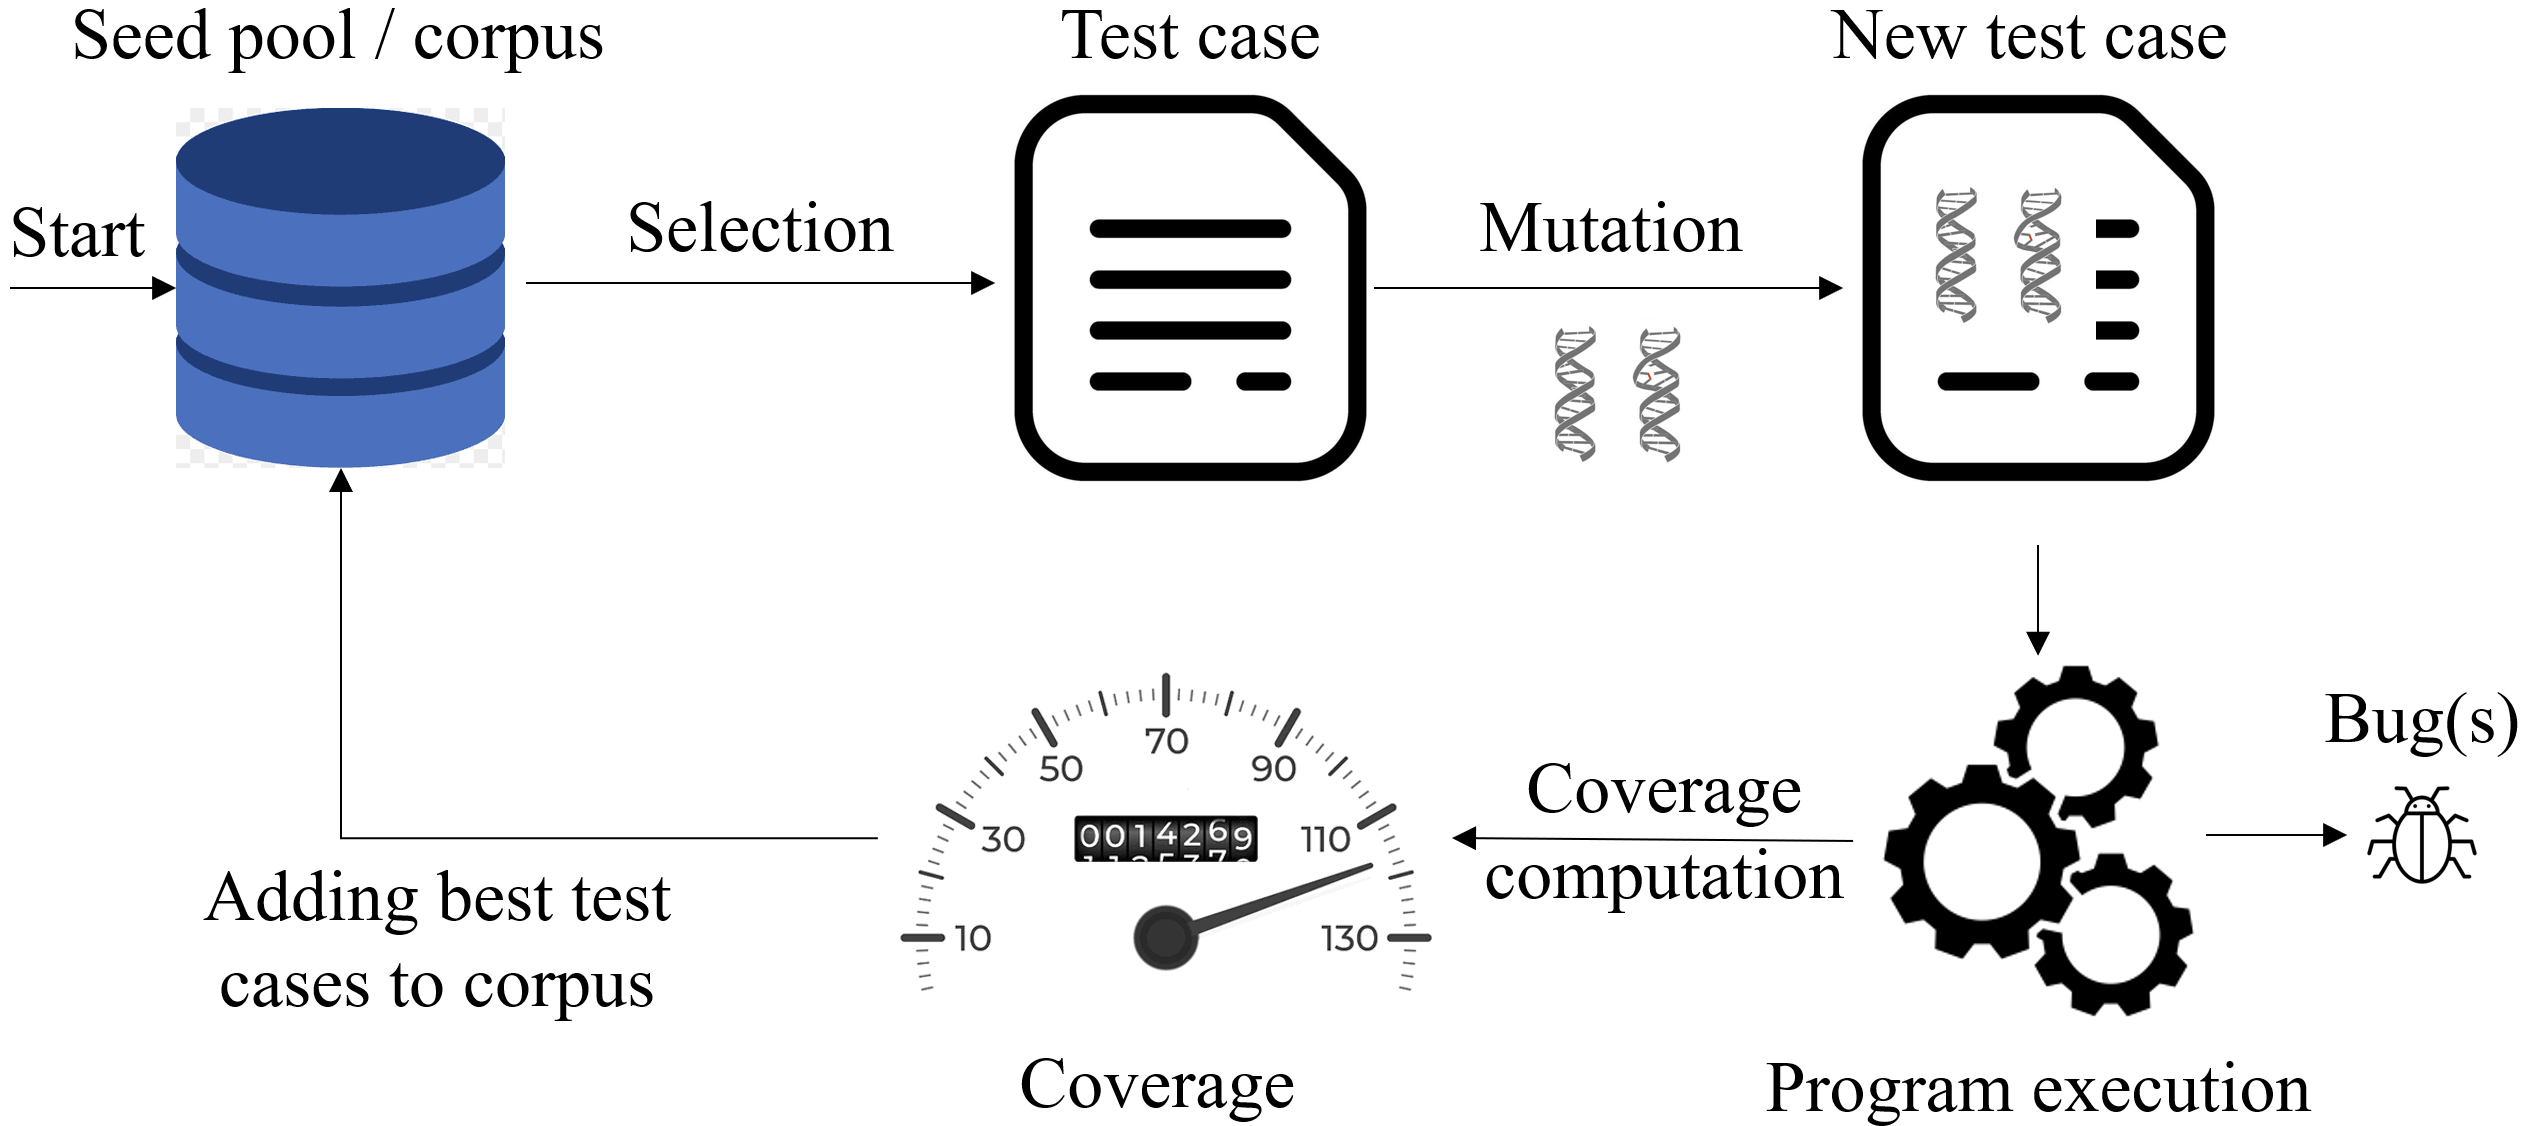
\includegraphics[width=3.25in]{coverage-fuzz.png}
        \vspace{-18pt}
        \caption{Traditional Coverage-Guided Fuzz Testing}
        \label{fig:coverage-fuzz}
    \end{minipage}%
    \begin{minipage}{0.5\textwidth}
        \centering
        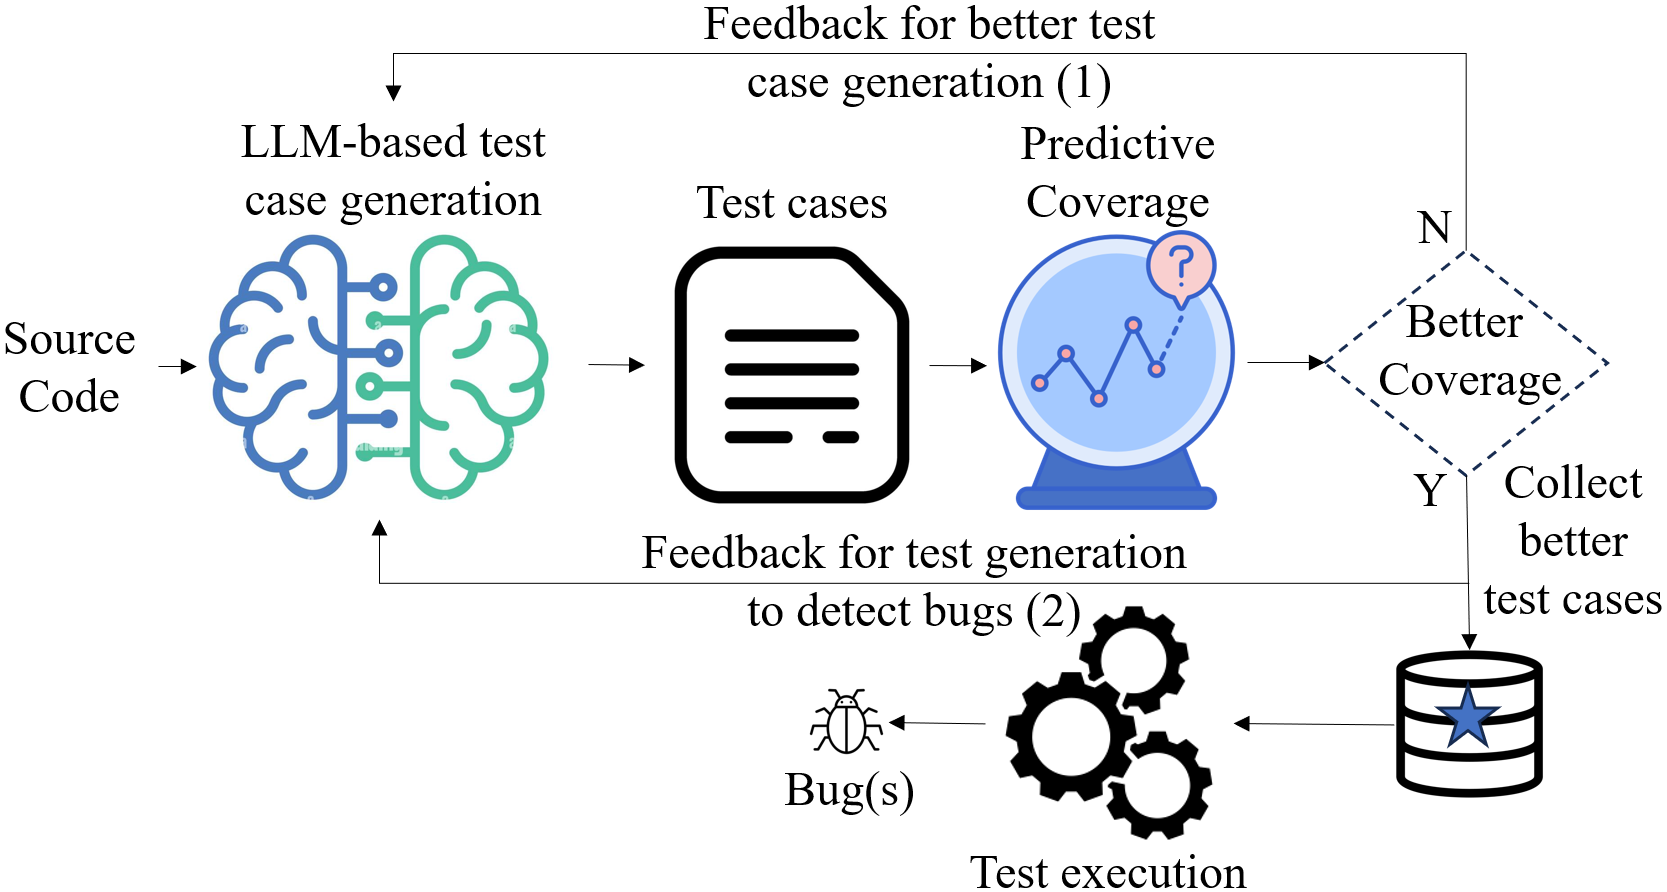
\includegraphics[width=3.3in]{fuzzwise2.png}
        \vspace{-18pt}
        \caption{Predictive Coverage-Guided Intelligent Fuzzing}
        \label{fig:fuzzwise}
    \end{minipage}
\end{figure}

%\begin{figure}[t]
%\begin{center}
%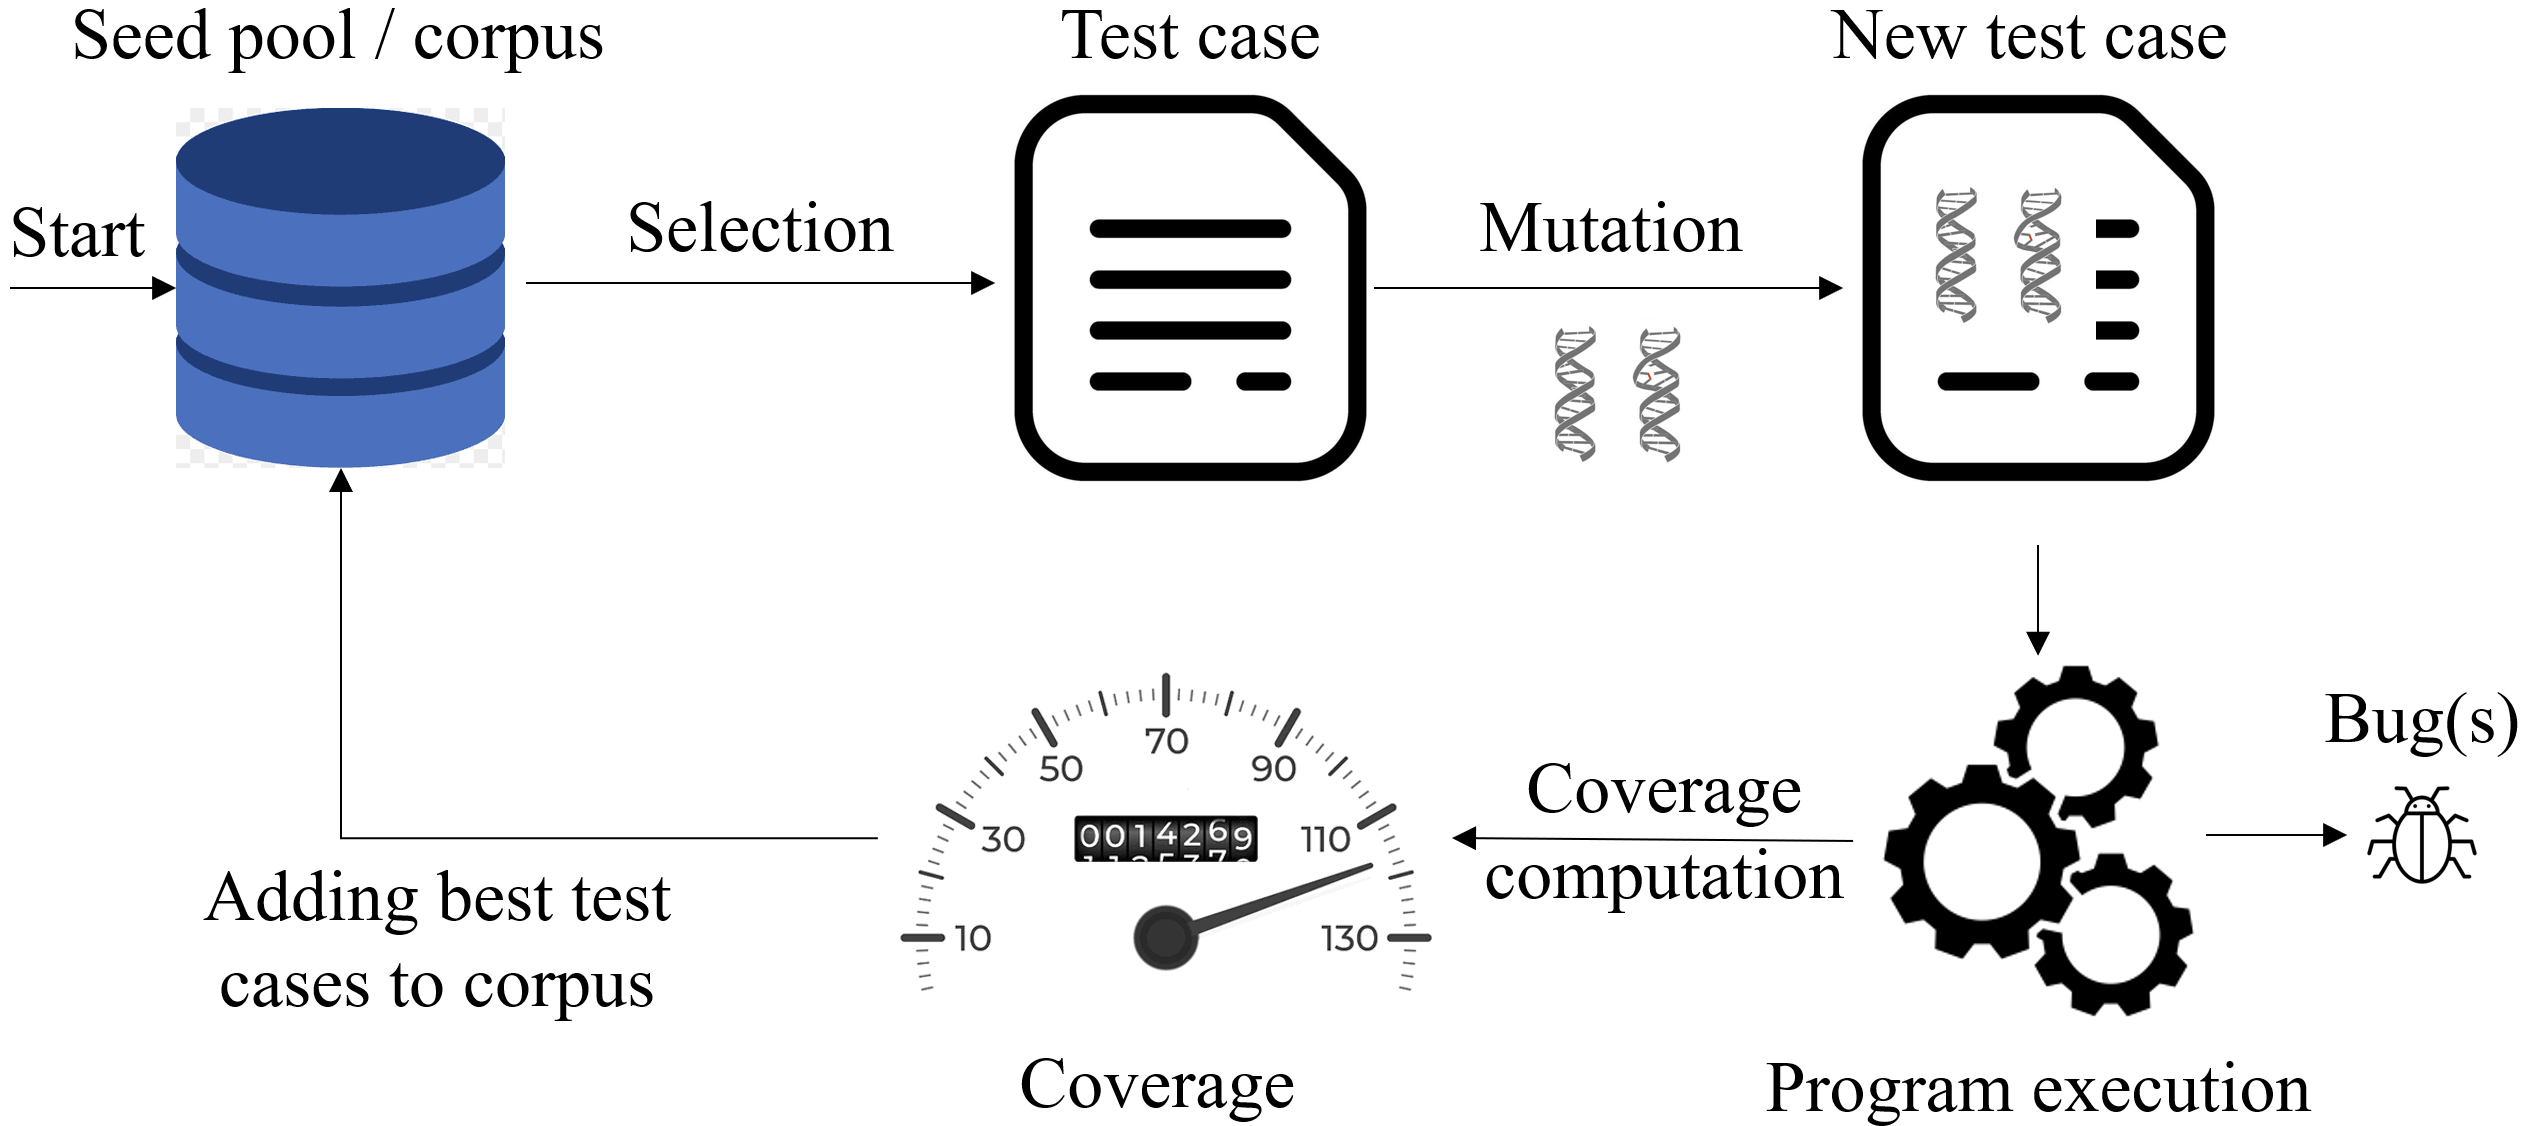
\includegraphics[width=3.4in]{coverage-fuzz.png}
%\vspace{-6pt}  
%\caption{Predictive Coverage-Guided Intelligent Fuzzing Framework}
%\label{fig:coverage-fuzz}
%\end{center}
%\end{figure}

%\begin{figure}[t]
%\begin{center}
%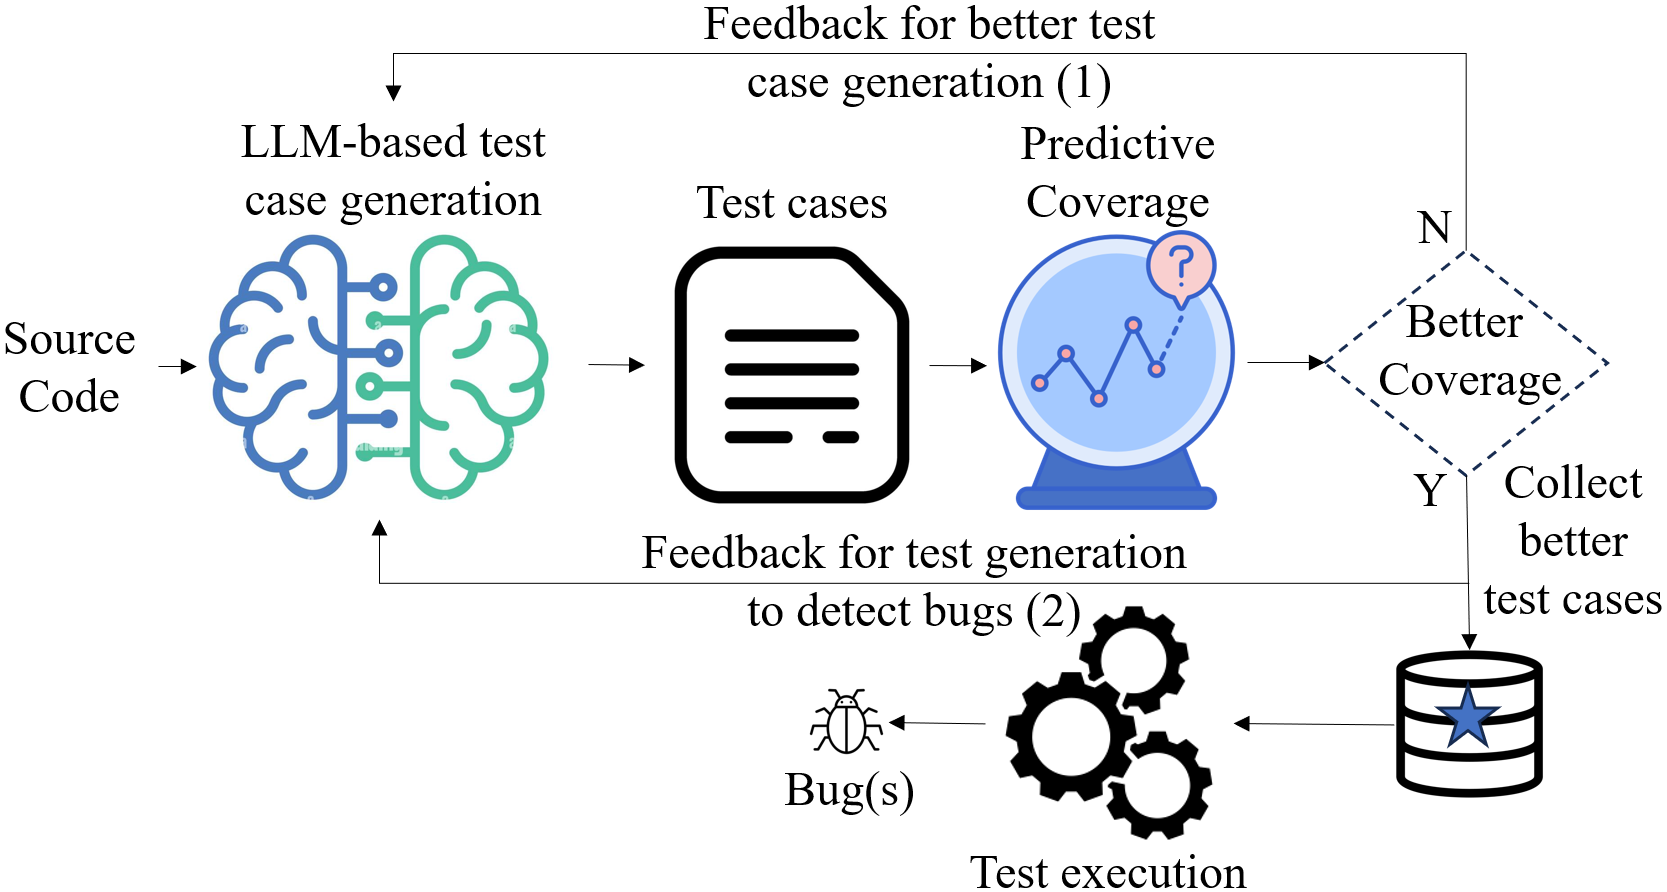
\includegraphics[width=3.5in]{fuzzwise2.png}
%\vspace{-15pt}
%\caption{Predictive Coverage-Guided Fuzzing Framework}
%\label{fig:fuzzwise}
%\end{center}
%\end{figure}

\subsection{Predictive Coverage-Guided Fuzzing Framework}

In this work, we propose {\tool}, a predictive code coverage-guided
intelligent fuzzing framework without actual test execution
(Figure~\ref{fig:fuzzwise}). For an upfront test quality assessment,
our \underline{first idea} is to develop a Large Language Model (LLM)-based code
coverage prediction approach, CodePilot~\cite{forge24}, that estimates
the quality of the generated test cases with regard to their code
coverages. The preliminary work on code coverage prediction is
described in~\cite{forge24}. This predictive approach aims to
identify, prioritize, and execute only the test cases that are likely
to contribute to higher total code coverage, thereby conserving
computational resources in actual execution, and focusing testing time
on the areas that likely need further testing.

Our \underline{second fundamental concept} aims to tackle the challenges
associated with mutations and the seed corpus. Instead of relying on
the conventional approach of mutating tests and enhancing the seed
corpus, we propose leveraging a LLM to automatically generate test
cases for the given source code under test. Within {\tool}, the
feedback loop is activated subsequent to the prediction of code
coverage. Once our predictive code coverage module determines that a
generated test case does not contribute to a higher total coverage of
the current test suite, we reintroduce these cases to the LLM.
This process enhances the generation of test cases from the LLM with
the goal of covering more un-tested areas in subsequent cycles. This
is carried out in the feedback loop (1) (Figure~\ref{fig:fuzzwise}).

Once predictive code coverage module determines that~a generated
test case would contribute to achieving higher overall coverage, we
collect it into the current test suite. However, we defer their
execution at this stage. Instead, the framework proceeds to the second
loop (2), where it prompts the LLM to generate additional test cases
with the main goal of enhancing the probabilities of detecting bugs and
runtime errors.

To enhance both effectiveness and efficiency, we instruct the LLM to
generate multiple test cases simultaneously: one seed test case and
several ``close'' variants. This approach aims to exploit a
faulty area within the source code by producing test cases closely
related to the seed. As the second loop (2) starts, we
expect that the LLM will begin exploring a new faulty area in the
source code. This functionality mirrors the traditional approach of
using different seed test cases. By adopting this strategy, we aim to
address the ``plateau'' issue, where the fuzzing process becomes
stagnant despite generating numerous mutations. The process will
terminate once either the cumulative code coverage of the entire test
suite reaches 100\% or the predetermined time limit is reached.


%We have conducted several experiments to evaluate {\tool}. Our result
%in the FixEval dataset~\cite{haque2023fixeval} shows that within a
%time limit, {\tool} generates significantly less test cases (only
%about 0.0065\%), yet to detect more runtime errors than the
%conventional fuzz testing framework in Jazzer~\cite{jazzer}. {\tool}
%is more efficient in runtime error detection compared to the baseline:
%on average, {\tool} executed {\bf 163} generated test cases to detect a
%runtime error, while Jazzer executed {\bf 4,217,067} test cases per error,
%thus showing that {\tool} saves execution time over Jazzer for
%ineffective test cases. The ratio between the number of effective test
%cases over the total number of generated ones for {\tool} ({\bf 0.48})
%is also higher than that of Jazzer ({\bf 0.41}), showing that {\tool}
%produces more effective, higher-quality test cases. Our result also
%shows that it took significantly less number of test cases for {\tool}
%to detect the next runtime error from the previous one than Jazzer.
%Moreover, we show that {\tool} overcomes the coverage plateau better
%than Jazzer. Importantly, the code coverage prediction module is
%sufficiently accurate in which {\bf 67\%} of test cases predicted by
%{\tool} as enhancing the coverage are indeed effective in doing so.

%The key contributions of this paper include:

%{\bf 1. {\tool}:} a novel predictive code coverage-guided fuzz testing
%framework that leverages predictive code coverage to conserve
%computational resouces in execution.

%{\bf 2. LLM-based Test Case Generation:} we leverage LLM to analyze the
%given code and generates the test cases with the feedback loops to
%iteratively improves the test case quality.

%{\bf 3. Extensive Empirical Evaluation:} to demonstrate that {\tool} is
%more effective and efficient than the baseline fuzzing models. Data
%and code is available at~\cite{fuzzwise-website}.









\subsection{Research Objectives and Anticipated Results}

\begin{figure}[t]
    \centering
%    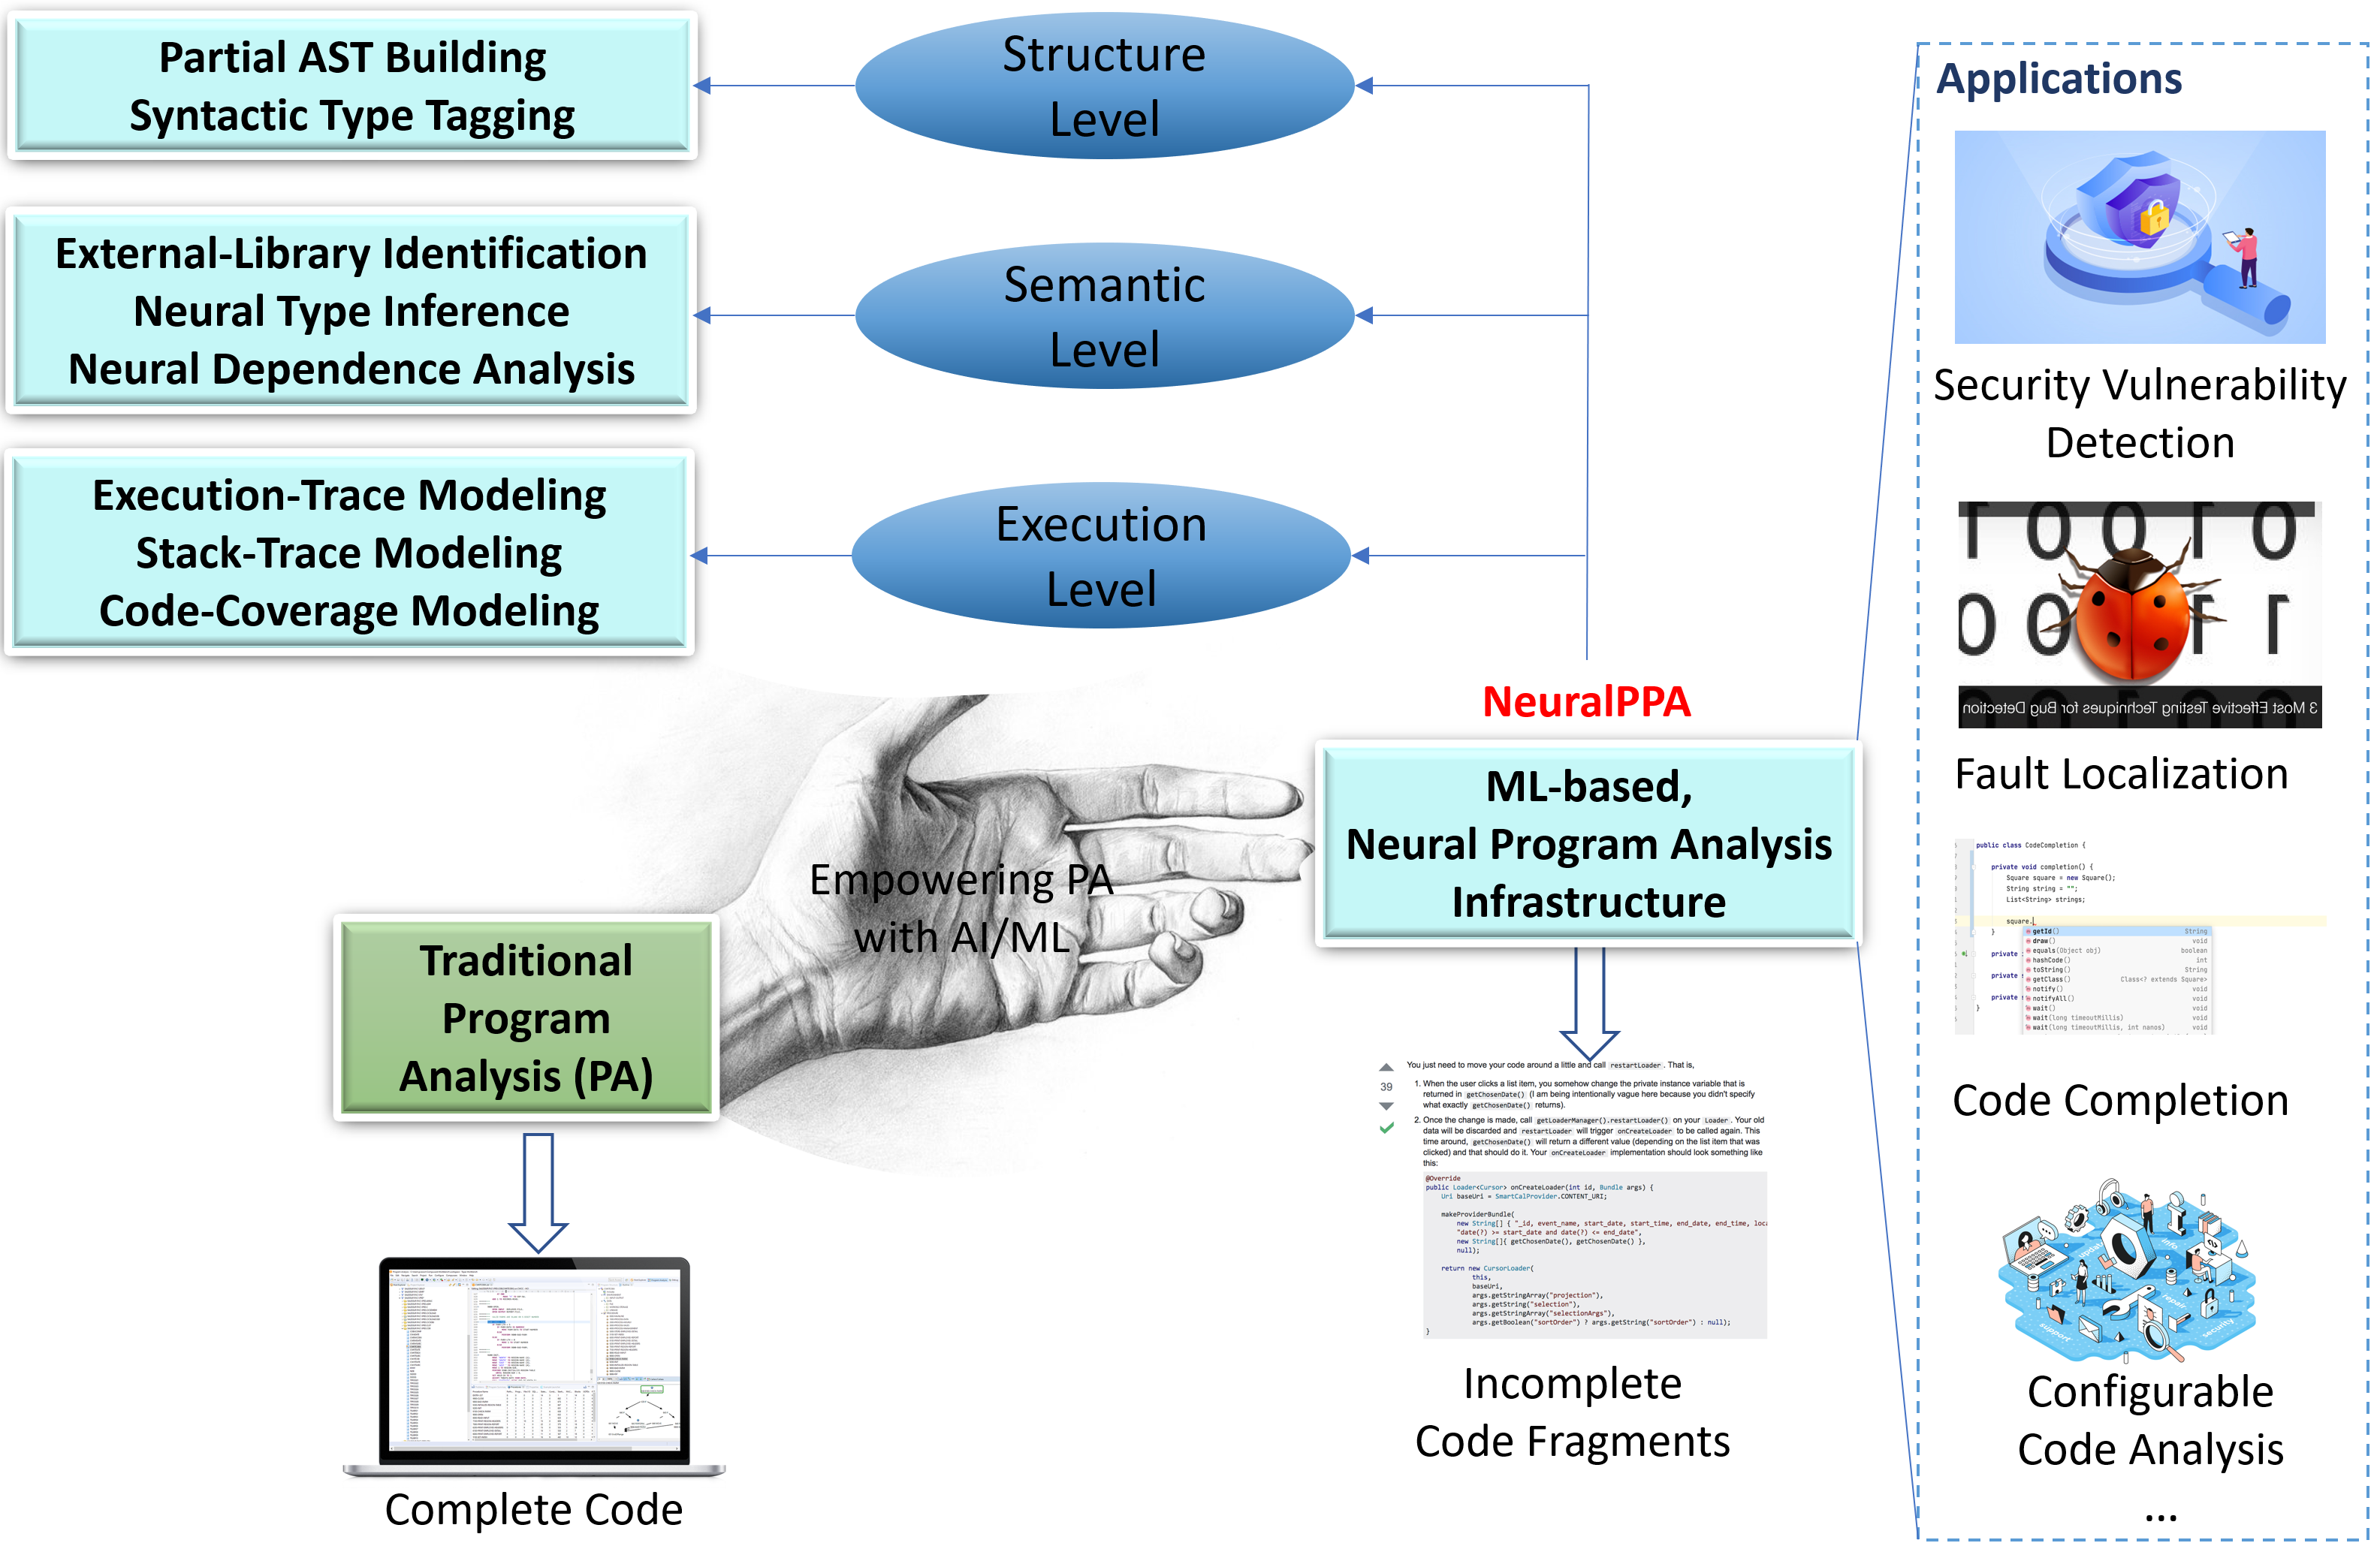
\includegraphics[width=0.83\textwidth]{graphs/neuralppa}
%    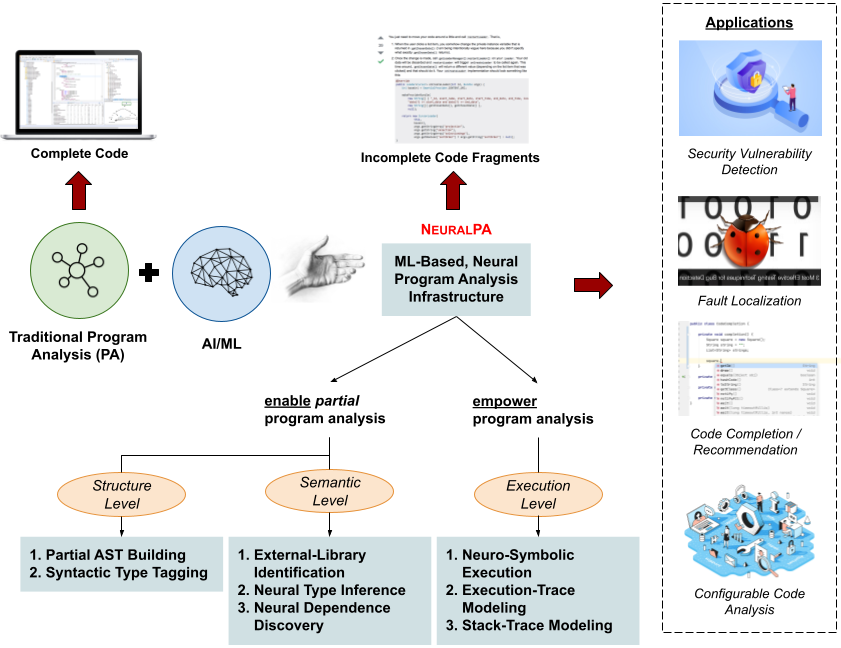
\includegraphics[width=0.92\textwidth]{figures/infra-design-3.png}
    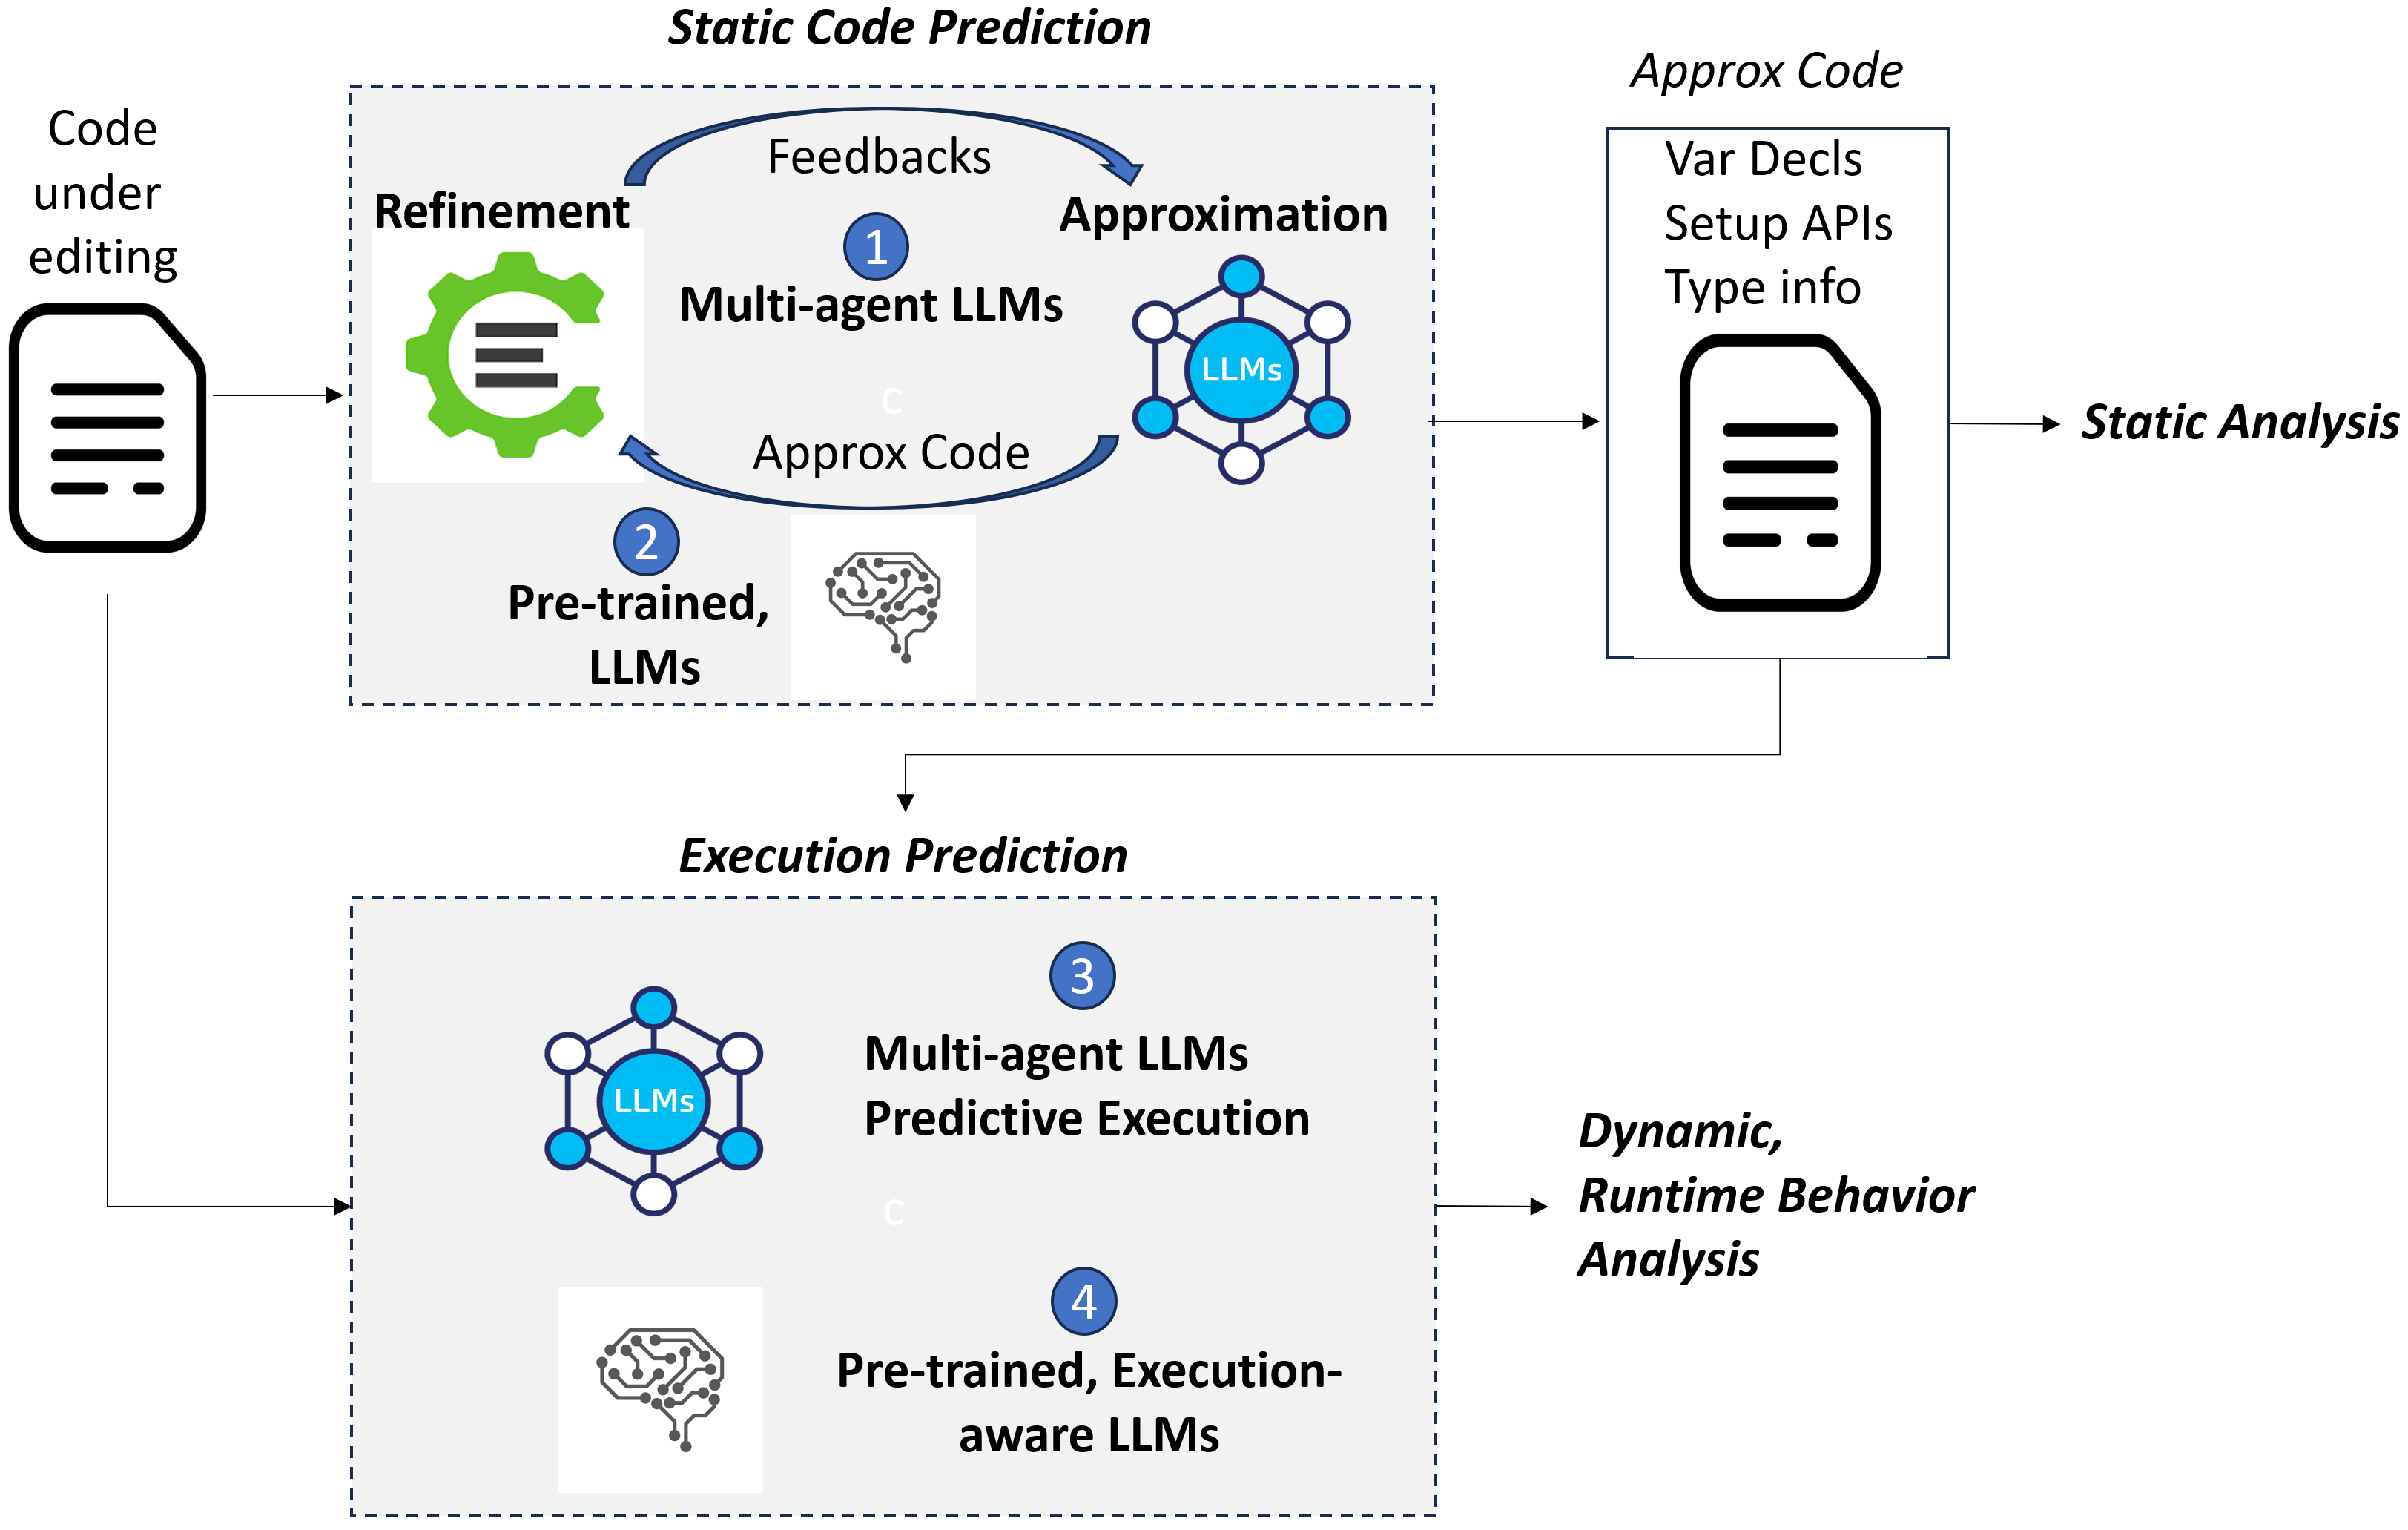
\includegraphics[width=0.92\textwidth]{overview.png}
    \vspace{-10pt}
    \caption{Predictive Program Analysis: Learning to Analyze Program Behaviors for Incomplete Code}
    \label{fig:arch}
\end{figure}


In this proposal, we seek to advance the state-of-the-art in
traditional program analysis by means of {\tool}, a Predictive Program
Analysis framework, with the goal to support program analysis for
incomplete/inexecutable code. We aim to establish {\em a scientific
  foundation, novel methodologies, frameworks, models, and algorithmic
  solutions for predictive program analysis} with the following focus
areas:



(1) {\bf enabling static program analysis on incomplete code}, and

(2) {\bf supporting predictive analysis for dynamic program behaviors}.

%\noindent Figure~\ref{fig:arch} illustrates the framework for {\tool},
%which will allow the construction of efficient program analysis
%techniques for (partial) code, also based on which downstream vulnerability detection and assessment applications can be built.

Our predictive program analysis framework is also beneficial in other
scenarios in addition to programming assistants. Predictive execution
is not aimed to replace actual execution. Rather, it offers a solution
where the actual execution is impossible, specifically in the
scenarios 1) where the complete source code of the implementation is
not available, or 2) where the analysis or approximation on the
behavior of the code is needed/desired without actual execution and
some degree of inaccuracy in prediction is tolerable.  First, the
first scenario can be exhibited in several examples, e.g., in the code
snippets in Stack Overflow or GitHub gist. They often miss contextual
information, such as imports and definitions of variables and
functions. It can take a great deal of efforts to integrate such code
snippets to a codebase.
%Horton and Parnin~\cite{horton2018gistable} reported that ``75.6\% of
%Python code snippets in gist require non-trivial configuration to
%overcome missing dependencies, configuration files, reliance on a
%specific operating system, or some other environment
%configuration''. Hossain {\em et al}~\cite{hossain2019executability}
%found that after installing the top 40~Python packages, the overall
%execution success rate for Stack Overflow Python code snippets is only
%27.9\% considering those running in either Python 2 or Python 3
%environments.
%Moreover, in~his keynote,
%Yahav~\cite{yahav2023fse} poses a need to approximate the execution of
%the incomplete code under editing in an AI-assisted programming
%environment.
Second, the instances of the second scenario can include the
analysis/approximation~of the behavior to check properties of
untrusted code or~to~detect bugs early. Moreover, even with complete
code, setting~up running environments for dynamic analysis is
undesired due to missing third-party dependencies and complex build
configurations.

The key philosophy that drives our work is that the analysis of
partial code can be learned from the analysis of entire programs in
the wealth of information obtained from ultra-large-scale, open-source
software repositories. To accomplish these tasks, we propose the
following thrusts of research in {\tool} (Figure~\ref{fig:arch}):

\noindent \textbf{Thrust 1. LLM Multi-agents and Pre-trained Language Models for Static Analysis on Incomplete Code.} ({\em Section~\ref{sec:thrust1}})

We advocate for a novel paradigm, called {\bf predictive program
  analysis}, which operates on the principles of {\em
  Approximation-Refinement} for Analysis. In the Approximation phase,
a large language model (LLM) acts as a machine learning (ML) agent to
fill in missing information within incomplete code. The missing
information that will be filled by the LLM could be manifested {\em
  explicitly}, e.g., in terms of missing variable declarations, setup
API method calls, import statements, and exception handling types, or
{\em implicitly}, e.g., in terms of missing type information of the
program elements, missing program dependencies, etc.

%Leveraging an LLM for this is advantageous due to its capability of code understanding.

A naive solution is to take whatever information the LLMs completed
and feed to a traditional program analysis technique as is. However,
researchers have shown that while LLMs are remarkable in code
generation with correct syntaxes, the produced code often contains
semantic errors and even do not compilable.  Thus, the Refinement
phase employs a program analysis (PA)-based agent to verify the
completed code output by the LLM. This PA-based agent utilizes the
compiler technology to ensure that the generated code is compilable
and consistent with used external libraries.  The iterative interplay
between the LLM-based agent and the PA-based agent continues until a
compilable code is achieved.
%If after a specified number of iterations the code remains
%uncompilable, human intervention may be sought for final resolution.
{\em Such interplay between the LLM and PA agents aims to enhance both the
recall and precision} of the analysis when comparing with the approach
using directly the PA technique on the incomplete code. We aim to
leverage {\em LLMs' expansive search capabilities} and {\em PA-based
  agents' semantic verification abilities}.
%The LLM is used to expand the candidate list of potential complete
%code for the current incomplete snippet, and PA is used to verify to
%make sure the validity of the chosen candidate. Subsequently,
%downstream program analysis techniques can be applied in the Analysis
%phase.
%It's important to acknowledge that the LLM may not always be capable
%of providing the exact missing information that developers would
%create when incorporating incomplete code snippets into their projects
%because each project might have its own . However, leveraging its
%proficiency in understanding code, we anticipate that it will fill in
%the gaps with the most probable information for the given incomplete
%code. Subsequently, following verification by the PA agent, the code
%is rendered complete and ready for analysis techniques to generate
%more accurate results in which without our framework, these techniques
%would be ineffective in handling incomplete code.
We propose a tandem solution that combines LLMs and PA agents to
leverage the strengths of both methodologies. This integrated approach
aims to optimize performance by harnessing the complementary
capabilities of LLMs and PA techniques. Specifically, the objective is
twofold: 1) to enhance recall compared to the PA-only solution (via
the Approximation phase), and 2) to maintain or even improve precision
beyond what can be achieved with LLM-only solution by integrating PA
techniques to ``correct'' the LLM's solution (via the Refinement
phase).


%One of the key foundations of {\tool} lies in its neural structural analysis component, which is built upon the well-defined structure and semantics of source code. This component serves two primary functions. Firstly, it draws upon the syntactic structures of comprehensive code samples from large-scale repositories in the training dataset. From this data, it constructs an abstract syntax tree (AST) that best encapsulates the syntactic arrangement of the provided partial code, aiming for the highest likelihood or probability. In contrast, existing program-analysis-based partial parsing methods~\cite{ppa08} rely on heuristics derived from the syntactic rules of programming languages, lacking the capacity to rank or score potential candidates. The second task of this component involves labeling code tokens with the corresponding types of syntactic units, encompassing statement types (\code{if}, \code{for}, etc.), variables, fields, methods, classes, and more. Both tasks can be efficiently executed through our dual-learning-based approaches.

%Source code has a well-defined structure and semantics. Thus, the basic infrastructure in {\tool} is the neural structural analysis component, which primarily has two tasks. First, it learns from the syntactic structures of the complete code in the training dataset collected from large-scale code repositories, to derive the abstract syntax tree (AST) that best represents the syntactic structure of the given partial code, i.e., with the highest likelihood/probability. The existing program-analysis-based partial parsing approaches~\cite{ppa08} rely on the heuristics on the syntactic rules of the programming languages. They do not give us any ranking or scores among the potential candidates. The second task of this component is to tag the code tokens with the types of the syntactic units including the statement types (\code{if}, \code{for}, etc.), variables, fields, methods, classes, etc. Both of the tasks can be performed with our learning-based approaches in a dual-learning manner.
  
%\vspace{3pt}
%\noindent \textbf{Thrust 2. Pre-trained Large Language Models for
%  Incomplete Code Static Analysis} ({\em Section~\ref{sec:thrust2}})
%Our work is driven by the fundamental belief that insights gained from
%training by complete programs within vast repositories of
%ultra-large-scale, open-source software can inform the analysis of
%partial code.

While exploring LLM-based multi-agent solution, we also aim to develop
smaller models via pre-trained language models. Our work is driven by
the fundamental belief that insights gained from training by complete
programs within vast repositories of ultra-large-scale, open-source
software can inform the analysis of partial code. Hindle {\em et
  al.}~\cite{naturalness-icse12} have shown that code has high
repetitiveness and predictability and can be captured well by
statistical models. Thus, we expect to build ML/DL models to learn
from those repositories.



%The basis components for several analysis techniques on the semantics
%of the program could tentatively include the following (more
%components will be added as the project evolves):

%1) the identification of the APIs of the external libraries in the
%external references in the partial code: this is needed because the
%partial code contains the undeclared reference and/or
%declaration/reference ambiguity without explicit declaration of the
%APIs in the external libraries. The knowledge on the external
%libraries enables more precise analysis of the code snippets.

%2) the inference of the type information for the entities in the
%partial code: due to the ambiguity in the declaration, the types of
%the variables and statements are not always obviously
%identified. Thus, the type inference is a basic service within
%{\tool}.

%3) the inference of the program dependencies among the statements in
%the partial code: several program analysis techniques are based on the
%program dependencies, which are not always obtainable due to the
%incompleteness of the given code fragment.

%4) Program slicing: program slices are important in both code
%understanding and program analysis for code snippets. That allows the
%analysis on the statements affecting or to be affected by a specified
%variable. All traditional program slicing techniques require the code
%to be complete.

\vspace{3pt}
\noindent \textbf{Thrust 2. LLM Multi-agents and Pre-trained
  Language Models for Predictive Execution.}  ({\em
  Section~\ref{sec:thrust2}})

We advocate for an execution paradigm called predictive execution. In
predictive execution, with a specific input, the execution is not
carried out with the computer performing the instruction in the
program. Instead, a trained machine learning model predicts the
execution steps and as a result, the execution trace corresponding to
the input is derived without actual execution.

By simulating program behaviors and outcomes without running the code,
these approaches provide valuable insights into the program's
potential runtime characteristics. Here are some benefits of
predictive execution. First, early error detection: predicting program
executions allows for the early detection of errors and potential
vulnerabilities before executing the code. By simulating different
execution paths and scenarios, predictive execution can enable the
dynamic analysis tools to identify potential issues such as null
pointer dereferences, memory leaks, or buffer overflows without the
need to execute the code in a real-world environment. This early error
detection helps developers catch and fix bugs more efficiently,
reducing the likelihood of critical issues in production. Second,
dynamic analysis techniques that predict program executions play a
crucial role in security analysis. By simulating potential attack
scenarios and analyzing how the program behaves under different
conditions, these tools can identify security vulnerabilities such as
injection attacks, privilege escalation, or data breaches. Predictive
execution analysis helps security professionals assess the resilience
of software systems against various threats and vulnerabilities,
enabling proactive security measures and robust defenses. Finally,
predicting executions provides developers with a deeper understanding
of their code's behavior without the need for actual execution. By
simulating program flows and interactions, tools can uncover hidden
dependencies, identify unexpected behaviors, and reveal complex
program dynamics. This insight into program behavior helps developers
better comprehend their code, debug more effectively, and make
informed design decisions.

In addition to the LLM-based multi-agent solutions, we also explore the
pre-training language models. We aim to teach a smaller model to analyze
the runtime behaviors via the learning from those of the open-source,
complete programs in execution.


%Symbolic execution is a means of analyzing a program to determine what
%inputs cause each part of a program to execute. Symbolic execution
%performs executing a program abstractly, so that one abstract
%execution covers multiple possible inputs, which are assumed to have
%symbolic values. We aim to explore the novel area in AI named
%neuro-symbolic learning, which seeks to combine traditional
%rules-based AI approaches with modern deep learning techniques.  We
%will leverage traditional program analysis rules to enhance the
%learning of the characteristics on the execution of the partial code
%fragment.

\vspace{3pt}
\noindent \textbf{Thrust 3. Programming Assistant Applications with Predictive Program Analysis.}  ({\em Section~\ref{sec:thrust3}})


Our last thrust of research is aimed to demonstrate the usefulness of
our solution in different programming assistant applications: 1)
vulnerability detection, 2) dynamic slicing, and 3) debugging and
error detection.



%2) fault localization, and 3) code completion.

%\vspace{3pt}
%\noindent \textbf{Thrust ???. Neural Execution Analysis Infrastructure.}
%({\em Section~\ref{}}) All the dynamic analysis techniques require the
%analysis and understanding of the execution. However, for an
%incomplete code, we first need to design a component that can wrap
%around the given code fragment with the minimum code so that the code
%fragment can be executed. When the code is executed, we also need the
%approaches that represent the executed statements and their relations,
%model the execution and stack traces, and model the code coverages
%for an execution.




%Toward this theme, in our preliminary work, we developed DeepPDA
%(Section~\ref{sec:deeppda}), a neural network-based partial program
%dependence analysis approach that learns to derive the program
%dependencies for any code fragments (i.e., both complete and
%incomplete). In our preliminary empirical evaluation, we intrinsically
%evaluated it on Java and C/C++ programs. We trained DeepPDA on
%complete code. For testing, we treated each method individually and
%chose a consecutive portion within the method to predict the program
%dependencies, and compared them against the actual
%dependencies. Overall, DeepPDA predicts CFGs/PDGs in Java with
%an F-score of 94.29\%, and in C++ with an F-score of 92.46\%. As
%another preliminary work (Section~\ref{sec:statype}), we also
%developed an approach to derive the data types of the variables in the
%code snippets. We treat the problem as statistical machine translation
%from source code with partially qualified names to source code with
%full names. Our preliminary evaluation on StackOverflow posts shows
%that our technique achieves high accuracy with 97.6\% precision and
%96.7\% recall in deriving data types in code snippets.

%We also test the usefulness of the PDGs predicted by DeepPDA (i.e.,
%PDG*) on the downstream task of method-level vulnerability
%detection. We discover that the performance of the vulnerability
%detection tool utilizing PDG* is only 1.1\% less than that utilizing
%the PDGs generated by a program analysis tool.
%We also report the detection of 14 real-world vulnerable code snippets
%from StackOverflow by a learning-based vulnerability detection
%tool that employs the PDGs predicted by DeepPDA for these code snippets.

\begin{table*}[t]
	\vspace{-15pt}
\begin{center}
{\footnotesize{
\begin{tabular}{cc}
\begin{tabular}[t]{|p{0.2in}|p{2.95in}|} 
\hline
\multicolumn{2}{|>{\columncolor[gray]{0}}c|}{\textcolor{white}
{\bf Year 1 Project Milestones \& Deliverables}}\\
\hline 
\hline
\multicolumn{2}{|c|}{\bf T1. LLM Multi-agents for Static Analysis}\\
\hline
{\bf 1.1} & LLM Multi-agent framework\\
{\bf 1.2} & LLM Multi-agent and Static Analysis\\
{\bf 1.3} & Pre-trained Language Models for Static Analysis\\
\hline
\hline
\multicolumn{2}{|c|}{\bf T1. Pre-trained Language Models for Static Analysis}\\ 
\hline
{\bf 1.4} & Pre-trained Language Models for Static Analysis\\
\hline
%\hline
%\multicolumn{2}{|c|}{\bf Integrate Code Synthesis into Tools}\\
%\hline
%{\bf 1.5} & \goalOneFour.\\
%\hline
\multicolumn{2}{c}{}
\end{tabular}
&
\begin{tabular}[t]{|p{0.2in}|p{2.95in}|} \hline
\multicolumn{2}{|>{\columncolor[gray]{0}}c|}{\textcolor{white}
{\bf Year 2 Project Milestones \& Deliverables}}\\
\hline 
\hline
\multicolumn{2}{|c|}{\bf T2. LLM Multi-agents for Predictive Execution}\\
\hline
{\bf 2.1} & LLM Multi-agents with Graphs\\
{\bf 2.2} & LLM Multi-agents with Execution\\
%{\bf 2.3} & Integrate Evaluation Framework into Design Environment\\
%{\bf 2.4} & Evaluate CRL Framework with Existing Models\\
%{\bf 2.3} & \goalTwoThree.\\

\hline
\hline
\multicolumn{2}{|c|}{\bf T2. Pre-trained Language Models for Predictive Execution}\\ 
\hline
%{\bf 3.1} & Design New Code Representations and Learning Models.\\
{\bf 2.3} &  Pre-trained Language Models for Predictive Execution\\
%{\bf 2.4} & Advance FL and RT-CI Approaches.\\
%{\bf 2.5} & Advance Regression Testing in CI Approaches.\\
%{\bf 2.5} & Advance APR Approaches with Framework.\\
\hline
%\hline
%\multicolumn{2}{|c|}{\bf Community Involvement: Capacity Building}\\
%\hline
%{\bf 2.4} & \goalTwoFour.\\
%{\bf 2.5} & \goalTwoFive.\\
%{\bf 2.6} & \goalTwoSix.\\
%\hline
\multicolumn{2}{c}{}
\end{tabular}
\end{tabular}\\
\vspace*{-.3cm}
\begin{tabular}{c}\hline
\multicolumn{1}{|>{\centering\columncolor[gray]{0}}p{6.44in}|}{\textcolor{white}
{\bf Year 3 Project Milestones \& Deliverables}}\\
\hline
\end{tabular}\\
\vspace*{-.2cm}
\begin{tabular}{cc}
\begin{tabular}[t]{|p{0.2in}|p{2.95in}|}
\hline
\multicolumn{2}{|c|}{\bf T3. Programming Assistant with Predictive Analysis}\\
\hline
{\bf 3.1} & Dependency Analysis\\
{\bf 3.2} & Debugging and Error Detection\\
\hline
%\hline
%\multicolumn{2}{|c|}{\bf \goalTwo}\\ 
%\hline
%{\bf 3.3} & \goalThreeThree.\\
%\hline
\multicolumn{2}{c}{}
\end{tabular}
&
\begin{tabular}[t]{|p{0.2in}|p{2.95in}|}
\hline
\multicolumn{2}{|c|}{\bf T3. Programming Assistant with Predictive Analysis}\\
\hline
%{\bf 3.1} & Design New Code Representations\\
{\bf 3.3} & Dynamic Slicing\\
\hline
\multicolumn{2}{c}{}
\end{tabular}
\end{tabular}
\vspace{-15pt}
}}
\end{center}
\vspace*{-.3in}
%\caption{Tasks and Milestones. (Rep. = Representation)}
\caption{The 3-year schedule of Thrusts, Tasks, and Milestones of this proposal.}
%the schedule of Thrusts, Tasks, and Milestones of this proposal.
%\vspace{-10pt}
\label{tab:milestones}
\vspace{-10pt}
\end{table*}
%




%\subsection{Significance of This Proposed Project: NSF Merit Criteria}

%\section{Relevance to Secure and Trustworthy Cyberspace}

%This project will develop novel concepts, representations, algorithms,
%models, and tools to support early software vulnerability
%detection. It is transformative and directly help improve software
%quality with novel program analysis-based software security and
%vulnerability detection tools on code snippets.

\section{Intellectual Merits}

%The results of this project will be transformative and directly help
%improve software quality with novel program analysis-based software
%security tools.

\noindent \underline{{\bf Advance the state-of-the-art knowledge and
    understanding}}. Predictive program analysis infrastructure in Thrusts
1--3 will advance the body of knowledge and theoretical foundations
in the area of {\bf machine learning and AI for code}. Thrust 4 will also help advance the practical tools in software engineering.

\noindent \underline{{\bf Scientific foundation, creative/original
    research}}. (1) to enable the analysis on partial code, (2) to empower
the program analysis techniques on both (in)complete code,
and (3) to enable the applications of program analysis on incomplete
code such as runtime error and vulnerability detection for code snippets, debugging tools for code under editing, etc.

\section{Broader Impacts}

\underline{{\bf (1) Transformative and benefits to society}}. Our
results will be transformative and directly benefit to our society.
They will lead to increasing developers' productivity, software
quality \& reliability.  Our validation involves students and
professionals, promoting teaching, training, and learning of both {\bf
  program analysis} and {\bf machine learning} techniques that
have wide impacts in industry and academic communities.

\noindent\underline{{\bf (2) Foster other related research
    activities}}. Our results will foster {\em research activities in
  related fields of {\bf machine learning} and {\bf software security}},
and the applications in software security and reliability.
%We will produce theoretical concepts and techniques that are novel in
%deep learning, e.g., novel neural networks to model and learn for
%code.
%The applications of our neural program analysis in software
%engineering applications will advance software security and
%reliability.

%The collected {\bf large scale bug\&fix corpus} will be useful for
%software quality and reliability research.
%Innovations in CRL could be used to {\bf advance other SE tasks}. We
%will also develop {\bf novel DL-based bug detect-fix} approaches.


\noindent\underline{{\bf (3) Education, dissemination, and broader participation}} (Section~\ref{edu}). The
research will enhance the infrastructure for teaching/research via
tools and data sets for use by students and practitioners, and for
enhancement by researchers. We will provide related learning
modules for educators as well. It will include outreach activities for
undergraduate students, underrepresented groups, minorities, and women
in science.
%contribute novel
%teaching modules to our curriculum.
%Details will be presented in Section~\ref{edu}


\iffalse
\begin{itemize}
	\vspace{-5pt}
\itemsep-0.2em 
  \item {\bf Transformative and benefits to society}. Our 
    results will be transformative and directly benefit to our
    society. 
    They will lead to increasing developers' productivity
    and software quality \& reliability. 
    Our validation involves students and
    professionals, promoting teaching, training, and learning of bug detecting and fixing techniques that have wide impacts 
    in industry and academic communities.

%report

  \item {\bf Foster other research activities}. Our results will
    foster research activities in related fields of deep learning and
    software quality. 
    This project will produce theoretical
    concepts and techniques that are novel even in deep learning, e.g.,
    novel neural networks for modeling and learning code. 
    The collected large scale bug fixing corpus will be useful for software quality and reliability research in general.
    %e.g.,   code transformation. 
%    This project will also advance
%    the state-of-the-art research in large-scale program analysis with
%    deep neural network models.

%The representation for software security vulnerabili will be useful in
%research on software security, malware detection, vulnerability
%reports, and automatic security patching.


  \item {\bf Education, dissemination, and broader participation}.
  The research will enhance the infrastructure for teaching and
  research by providing tools and data sets for use by students and
  practitioners, and for enhancement by other researchers. We will
  provide related learning modules for educators as well. It will
  contribute novel teaching modules to our curriculum. Details will be
  presented in Section~\ref{edu}

%Details are in Section 4.

\end{itemize}
\fi
